\documentclass{amia}
\usepackage{graphicx}
\usepackage{pdfpages}
\usepackage{subfig}
\usepackage[labelfont=bf]{caption}
\usepackage[superscript,nomove]{cite}
\usepackage{enumitem}
\usepackage{multicol}
\usepackage{multirow}
\usepackage{booktabs}
\usepackage{wrapfig}

\begin{document}


\title{An Interactive Data Repository for Studying Risk Factors Associated with Pressure Ulcer Resulting from Spinal Cord Injury}

\author{Ningzhou Zeng$^{1,2}$, Steve Roggenkamp$^{1,2}$, Shiqiang Tao, PhD$^{1,2}$, Kath M.BogieD.Philabd$^{3,4,5}$, PhD, GQ Zhang, PhD$^{1,2}$}

\institutes{
  $^1$Institute of Biomedical Informatics, University of Kentucky, Lexington, KY\\
  $^2$Department of Computer Science, University of Kentucky, Lexington, KY\\
  $^3$Advanced Platform Technology Center, Louis Stokes Cleveland Department of Veterans Affairs Medical Center, Cleveland, OH\\
  $^4$Department of Biomedical Engineering, Case Western Reserve University, Cleveland, OH\\
  $^5$Department of Orthopaedics, Case Western Reserve University, Cleveland, OH\\
}

\maketitle

\noindent{\bf Abstract}

\textit{Pressure Ulcer (PU) and Deep Tissue Injury (DTI) are serious and common among those individuals with spinal cord injury (SCI), which come at tremendous personal and societal cost. Primary PU/DTI prevention plays a critical role in the first line of defense, while it is also challenging as there are many risk factors ranging from the individual’s environment to local tissue health to consider. Beside, there is limited guidance on how to prioritize based on individual cases along with the standardized clinical pratical guidelines. In this paper, we present the SCIPUDSphere - a bioinformatics platform, enables data extraction, storage, and analysis to provide clinical decision support and user interface providing a single point of web-based access to well-annotated and de-identified data generated from multiple domains within the Veterans Administration's VA Informatics and Computing Infrastructure (VINCI) electronic health records.}

\section{Introduction}
Pressure Ulcer and Deep Tissue Injury are serious and costly complications for some populations, such as those with spinal cord injury (SCI), who remain at high risk throughout their lifetimes. Clinical observations and research have demonstrated staggering costs and human suffering ~\cite{ref1,ref2,ref3}. In addition to the psychological distress and detrimental effects on quality of life (QoL) for the individual, chronic wounds place a significant burden on health care systems, with US costs estimated to be up to \$15 billion per year, with an individual PU costing as much as \$37,800 - \$70,000 to treat  ~\cite{ref4,ref5,ref6}.

Primary PU/DTI prevention seeks to prevent the initial incidence of any tissue damage, while secondary PU/DTI prevention seeks to decrease chronic recurrence of tissue breakdown for the individual ~\cite{ref7}. It has been estimated that PU prevention is approximately 2.5 times more economical than treatment ~\cite{ref8}. Clinical practice guidelines (CPG) provide best practice recommendations, however, the many recommendations in a CPG reflect the multivariate nature of PU/DTI management. There is limited guidance on how to prioritize based on individual cases. The Agency for Health Care Policy and Research (AHCPR) has long recognized that there is a significant need to increase education and quality improvement methods ~\cite{ref9}. Forward thinking tactics are essential for the development of effective PU/DTI management tools to address this major consequence of SCI and guide personalized best practices for each individual.

In order to successfully prevent and treat PU/DTI in the SCI population, it is essential to consider multiple risk factors because they contribute to the formulation of treatment and rehabilitation strategies ~\cite{ref10}. These factors involve multiple domains, from the environmental factors related to the location of the patient (inpatient/nursing home/community dwelling) to the individual’s tissue health profile (see Figure \ref{risk_factors}). These domains can interact, working in opposition or in concert. This complexity highlights the challenge of PU/DTI prevention and is indicative of the need for a holistic and systematic approach. However, the multifactorial nature of PU/DTI care planning strongly implies that a universal standard approach will fail for many patients. It is essential to recognize that every patient is an individual and that personalized care plans are essential for effective management [54,55,56]. Consideration of multi-scale risk factors ranging from environmental conditions to tissue damage provides a pathway to personalized PU/DTI prevention to improve the health and QoL for all Veterans with SCI.

However, the integration of PU/DTI risk data, ranging from the living environment and age to tissue blood flow, requires a robust and scalable informatics approach to cope with big-data challenges in volume and complexity. PU/DTI risk data is collected using systems with a variety of different sampling rates and resolutions, with non-standard (often proprietary) data formats. For example, the clinical and demographic data of interest in PU/DTI is collected in the electronic medical record (EMR) at annual evaluations or when the Veteran attends the outpatient clinic for wound care with clinical information coded and in free form clinical text notes. Conversely, tissue oxygenation data is collected during tissue health assessments at a rate of 5Hz in a standardized format. Thus data extraction, integrated data analysis and data sharing are complex and challenging problems in PU/DTI risk data.

In this paper we present a bioinformatics platforms, called SCIPUDSphere. SCIPUDSphere is a platform that enables data extraction, storage, and analysis to provide clinical decision support and user interface providing access to well-annotated and de-identified data generated from multiple domains. SCIPUDSphere uses a novel Spinal Cord Injury Pressure Ulcer and Deep tissue injury ontology (SCIPUDO) as the knowledge resource for processing specialized terms related to SCI, PU and DTI. The SCIPUDSphere enables extracting a tremendous amount of data from VA Informatics and Computing Infrastructure\cite{VINCI} and integrating PU/DTI risk data, ranging from the living environment and age to tissue blood flow. 

\section{Background}

\subsection{VA Informatics and Computing Infrastructure (VINCI)}
VA Informatics and Computing Infrastructure (VINCI) is an initiative to improve researchers' access to VA data and to facilitate the analysis of those data while ensuring Veterans' privacy and data security. VINCI hosts many datasets and provides many types of analytical applications. Researchers can access the VA data and tools for reporting and analysis in a secure Workspace called VINCI Workspace. VINCI provides EMR data storage for all healthcare encounters within the Veterans Health Administration (VHA), updated on a daily basis. 

\subsection{Preliminary development of SCIPUD}
The first generation SCIPUD was created at the Louis Stokes Cleveland VA Medical Center (LSCDVAMC) by a multidisciplinary team included a physician, staff nurses, physical and occupational therapists, a dietician, biostatisticians and a public health specialist. A literature review [47] together with consultations with clinical experts was conducted to determine PU risk factors under the categories of basic demographic information, SCI/D history, equipment, medications, co morbidities and environment. Data was obtained through retrospective chart reviews of persons with SCI/D admitted to the LSCDVAMC for PU care and extracted from the electronic Computerized Patient Record System (CPRS).

SCIPUD was established with longitudinal data including all admission time points during the initial study timeframe. All data was collected using standardized data collection forms reviewed by Spinal Cord Injury Disorder (SCI/D) clinical experts and pilot tested for accuracy and completeness of data. A data collection manual was also developed to ensure inter- and intra-rater reliability of data collection. The manual was used to train study personnel on the data collection form and chart review methods. Data collectors were trained prior to data collection to prevent misclassification of data in the clinical record. Data collection forms were completed independently by three study staff using the same patient for chart review. Data obtained by chart review was then compared between staff. All data collected was equivalent and accurate compared to the chart record. Oversight was provided by a content expert knowledgeable on CPRS and SCI/D to further ensure reliability of data.

Multiple factors known to be associated with PU development were assessed at the admission timepoint and entered in to SCIPUD. An initial study was carried out to investigate the significance of risk factors for rehospitalization (RHA) for severe (Stage III or IV) PU [48]. Using SCIPUD, we found that factors previously found to be predictive of initial PU development may not be predictive of RHA. Specifically, demographic factors showed no significant association with RHA, while clinical factors such as duration of injury and sub-optimally managed spasticity (SMS) were significantly associated with higher RHA. These preliminary findings provide indications of the ongoing need to develop and review adaptive PU/DTI prevention care plans.

\subsection{Specific Challenges of PU/DTI Prevention}

More than 200 risk factors for PU development have been reported for individuals with SCI [12], spanning multiple domains [13]. The Center for Medicare and Medicaid Services (CMS) has determined that severe (Grade III and IV) hospital-acquired PU are completely preventable ``never-events'' and have discontinued reimbursement [14]. However, the clinical reality is that many patients continue to develop significant chronic wounds, both in the community and in hospital. Patients in acute care hospitals have 33\% PU incidence rates, with prevalence rates up to 69\% [15,16]. On admission to skilled nursing facilities, PU prevalence ranges between 10\% and 26\% [17,18]. Veterans with chronic SCI have incidence rates VINCI data extraction provides this information Specialized clinical assessment - usually obtained from a seating clinic or PT assessment as high as 62-80\% [19,20] and 34\% will require at least three hospitalizations for treatment [21]. PU/DTI may lead to other serious medical complications, such as osteomyelitis, sepsis and even death.

Primary PU/DTI prevention is encouraged as the first line of defense [22]. CPGs developed to aid clinicians in this goal combine a balance of evidence based practice and expert opinion. There are multiple CPGs for PU prevention [23,24,25,26,27], each containing similar recommendations regarding risk assessment, prevention, PU assessment, measurement, treatment and documentation however they also contain significant differences. The major challenge with all CPGs is that there are many factors to consider (see Figure \ref{risk_factors}). For example, the updated CPG from the Consortium for Spinal Cord Medicine released in September 2014 contains a summary of over 25 recommendations to be followed by the care provider [27]. However, there is still limited guidance on how to prioritize for individual cases. It is very challenging and even unrealistic to expect every recommendation to be implemented concurrently, which can be overwhelming [13]. The relative importance of risk factors has not yet been investigated, limiting care planning and prioritization of interventions.

\begin{wrapfigure}{r}{0.5\textwidth}
  \begin{center}
    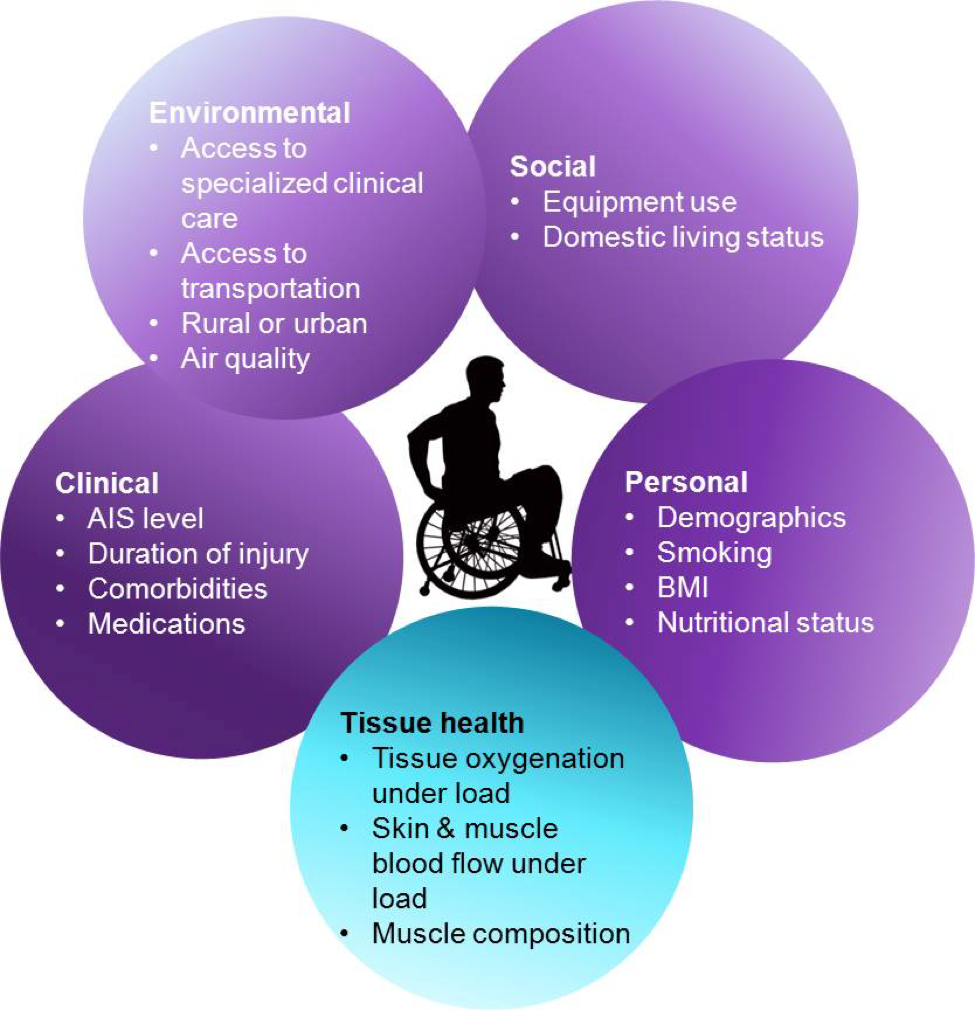
\includegraphics[scale=0.5]{pics/risk_factors.png}
  \end{center}
  \caption{Multiple risk factor domains contribute to PU/DTI risk}
  \label{risk_factors}
\end{wrapfigure}

\subsection{Physio-MIMI and OnWARD}
Zhang et al. have developed the Physio-MIMI cloud-based multi-modal data storage and access platform \cite{physiomimi}. Physio-MIMI creates a common user interface for data queries and enables development of compatible analytical tools and easier sharing of complex data from multiple domains to support collaborative clinical and translational research using diverse data types. 

Another system, OnWARD (Ontology-driven Web-based Research Data Capture) \cite{onward}, provides robust flexibility of input data storage in a relational database for detailed analysis. OnWARD can be quickly deployed and customized for any clinical study and has demonstrably eased the data entry burden in multiple clinical trials [53]. 

\section{Method}
The design of SCIPUDSphere involves three seamlessly integrated modules: SCIPUDO Ontology Support, Creation of the SCIPUDSphere environmental, social and clinical domain database and SCIPUDSphere User Interface. Agile development and agile project management methodologies were used to achieve a flexible and user-friendly web-based data management tool in the Ruby on Rails framework. Figure \ref{architecture} demonstrates the architecture of SCIPUDSphere system. 

\begin{figure}[h!]
  \centering
  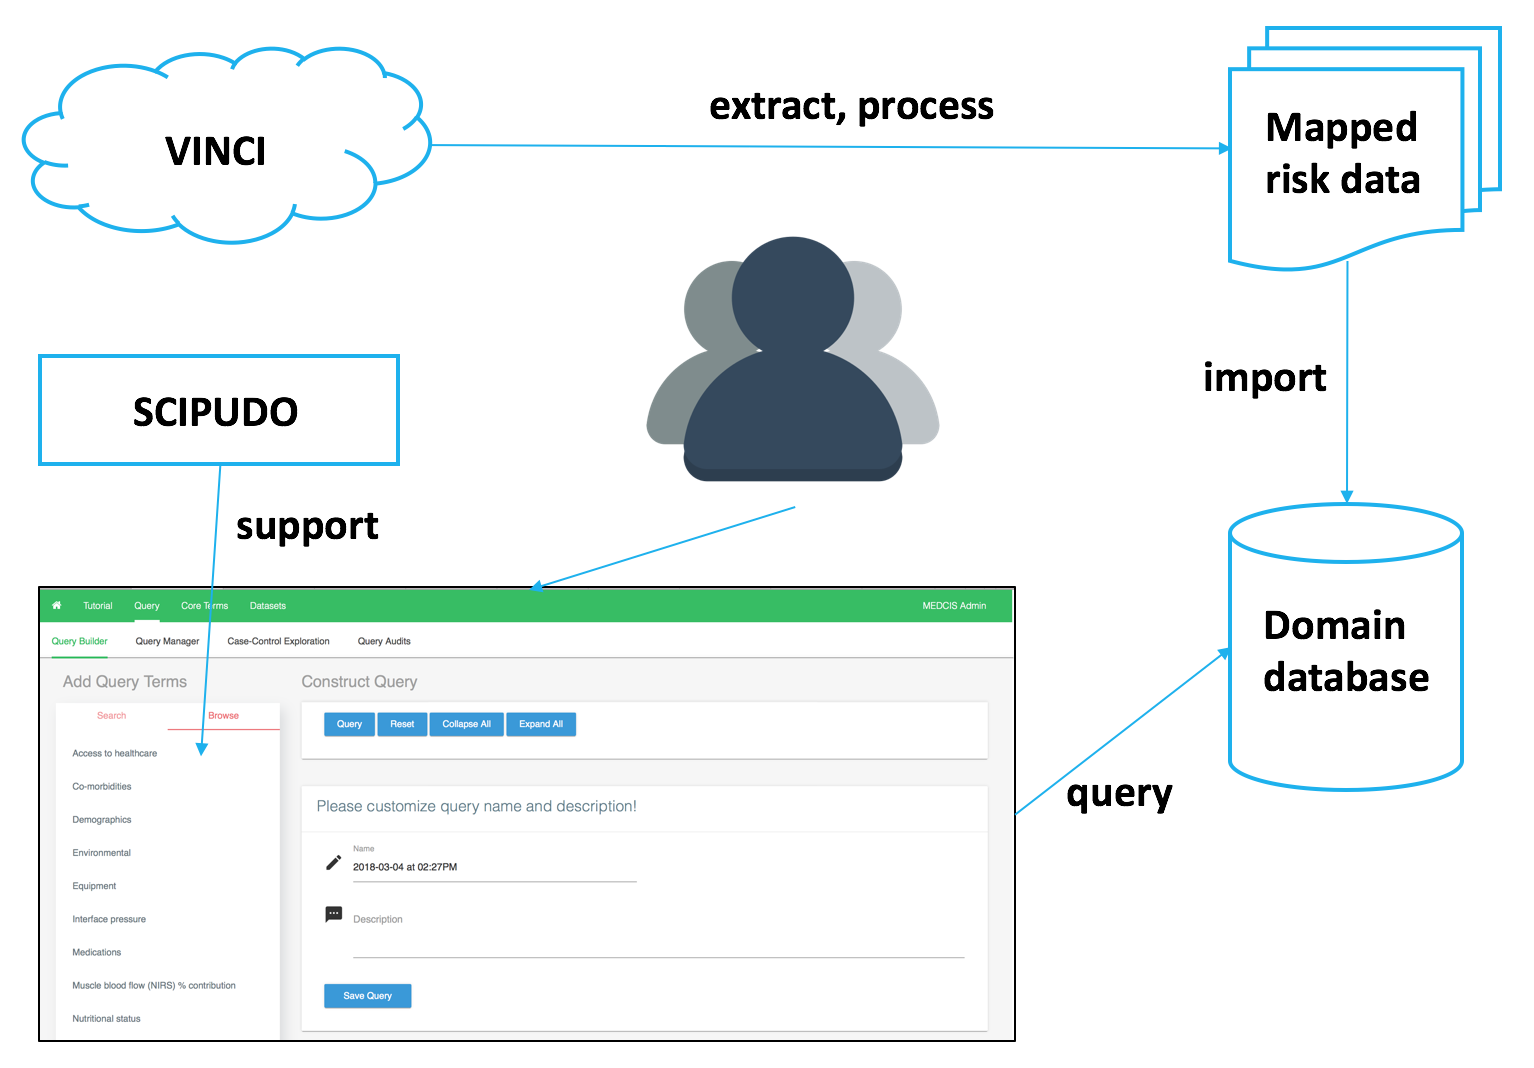
\includegraphics[scale=0.4]{pics/architecture.png}
  \caption{SCIPUDSphere System Architecture}
  \label{architecture}
\end{figure}

% Analysis of multiple PU/DTI risk factors requires a robust and scalable informatics approach to cope with challenges in volume and complexity. 
\subsection{SCIPUDO Ontology Support}
The dedicated domain ontology Spinal Cord Injury Pressure Ulcer and Deep tissue injury ontology (SCIPUDO) were created by reusing terminology from existing systems ranging from anatomy (SNOMED CT), disease classification (ICD-9 and 10), medication (RxNorm), and NINDS Data Elements. The SCIPUDO consists of a set of concepts (terms) in the PU/DTI domain and the relationships between the concepts. By employing the SCIPUDO, a standard set of terminology can be employed while allowing individual data contributors to maintain data according to their desired schema. Such ontology then can be plugged into our Physio-MIMI system to power the operation of SCIPUDSphere User Interface.

\subsection{Creation of the SCIPUDSphere environmental, social and clinical domain database}

In 2013, the Veterans Health Administration (VHA) launched a five year strategic plan with the goal of moving the healthcare system for our Veterans towards Personalized, Proactive, Patient-driven Health care, delivered across the continuum from prevention through tertiary care and end of life [31].  The VA has built a Corporate Data Warehouse (CDW) within VINCI to support this effort which contains detailed data about each encounter a patient has with a VA medical service.  We used this CDW as the source of patient data for our system.

Early in the project we needed do decide where to host our software.  We use an iterative development process where developers work closely with the end users to identify desired changes to the application.  Developers implement these changes and we update our application before repeating the cyle.  This lets us implement the most valuable features as quickly as possible.

Hosting it in VINCI's secure infrastructure would allow us to use identified data and provide quick updates to data. The disadvantages to this is only one member of the development team has credentials to access the VINCI and the process of implementing our incremental development process would be difficult.

Our study data are restricted to the dates ranging from October 1, 2010 to September 30, 2015, thus we expect few, if any, updates once we developed the proper queries.  We also have no requirements that need identified data, thus we could create deidentified records and export them.  We decided to host our application external to VINCI ased on these considerations and deidentify the data before exporting them from VINCI.

We ultilize MySQL as our SCIPUDSphere domain database and input data for the database are provided by synthesizing available EMR clinical data from VINCI, using a protocol based on our preliminary work. At our current stage of development a traditional database is sufficient to handle even more than 40,000 data entries as we don't have a column-intensive schema.

{\bf Data Extraction}. A member of the VINCI team provided a cohort of 36,628 VA patients having ICD9 codes associated with SCI.  Our study is limited to interactions with patients between October 1, 2010 through September 30, 2015, after which the VA converted to ICD10 coding.  We identified twelve tables containing identified patient data and queries of these tables provided 18,808,408 records containing ICD9 codes for 36,581 individuals.  We filtered this table to produce a table with 76,553 records containing 66 ICD9 codes related to SCI for 36,580 individuals and another table containing 153,930 records of 32,396 individuals with a total of 216 ICD9 codes for comorbidities included in our study.

We needed to deidentify this data to comply with HIPAA and VA requirements.  We accomplished this by computing the SHA256 hash for a unique identifier assigned by the VA to each patient and reporting the first and last year within the study period and the number of times the ICD9 code was recorded for the individual in this period.  Using SHA256 hashes as patient identifires allows us to assemble data from multiple sources as long as we can reliably generate the same hash for a given patient.

We also extracted demographic data for the patients in our cohort.  This data contains the age, sex and marital status of each patient..  The age is computed at the time of the patient's first encounter within the study period of this project and recorded as years.  All ages 90 and over are assigned a single value to comply with the HIPAA safe harbor standard.  We found 283 individuals of age 90 and above in our data. The resulting table contains 38,068 records with the extra records compared to the number of patients resulting from multiple values being recorded for race or marital status.

We are still researching the discrepancy between the number of patients contained in the original cohort provided by VINCI and the number of patients for which we have data.  We have found 4 test patients in the original cohort, that is, ``patients'' who have records in the system that do not exist but provide data quality checks.  We have removed these from our data.  That leaves 43 patients in the original cohort for which we do not have data.  We are investigating whether we should include additional CDW tables in our search or if their dates of encounters fall outside of the dates of our study or some other reason.

{\bf Data Processing}. The extracted data from the VINCI data are stored as a deidentified .csv format file. Prior to importing data into the SCIPUDSphere User Interface, we need to process the data in order to identifier the comprehensive domains for categorical risk factor and handle the missing value. After acquring the comprehensive domains for categorical risk factors, we then mapped the data into corresponding domains value and saved these data into new CSV files. Finally, we imported the mapped data into the SCIPUDSphere User Interface.

{\bf Summary}.

\begin{table}[!ht]
\centering
\caption{Extracted Risk Data from VINCI}
  \begin{tabular}{|l|l|l|l|}
  \hline
    \textbf{Dataset}  & \textbf{Data Records} & \textbf{Patients} \\ \hline
    Demographic            &  38,068  & 36,623 \\ \hline
    Co-morbidities         & 153,930  & 32,396 \\ \hline
    Patient SCI diagnosis  &  76,553  & 36,580 \\ \hline
    Total & 268,562 \\ \hline
  \end{tabular}
\end{table}

\subsection{SCIPUDSphere User Interface}
Validated extracted data are collated using our established standard data collection forms and imported to the Physio-MIMI based integrated PU/DTI risk assessment SCIPUDSphere platform. The Physio-MIMI backbone will provide extensible, scalable, and high performance data management for storing and accessing rapidly large volumes of data. Reliable data storage through automated data replication and data integrity verification will ensure consistent data availability and effective disaster recovery with off-site data backup. Data quality assurance and metadata version control will be managed using a combination of GitHub, JSON, and the open-source NSSR data management environment [63]. A visual query interface is adapted from OnWARD to allow all clinicians to directly query the PU/DTI risk data via a set of easily usable visual widgets that will be directly populated with the SCIPUDO classes to allow clinicians to flexibly construct queries, specific to the patient. All patient data are stored in a firewall protected secure environment with role-based access control and audit-trail logging. 

The ability of interface to query risk data is dependent on the ontological mapping. The Query Builder provides the user interface to formulate the necessary patterns - allowing the construction of a logical query. The logical query is translated into a local database query based on the mapping between the ontology model and the database specific data model dynamically.

\section{Preliminary Results}
In this section, we will first present the preliminary results for data extraction, integration in our domain database, then show the query interface. 

\subsection{SCIPUDSphere User Interface}
We adapted the domain ontology SCIPUDO into the highly adaptable Physio-MIMI system and developed SCIPUDSphere User Interface. 

\begin{figure}[h!]
  \centering
  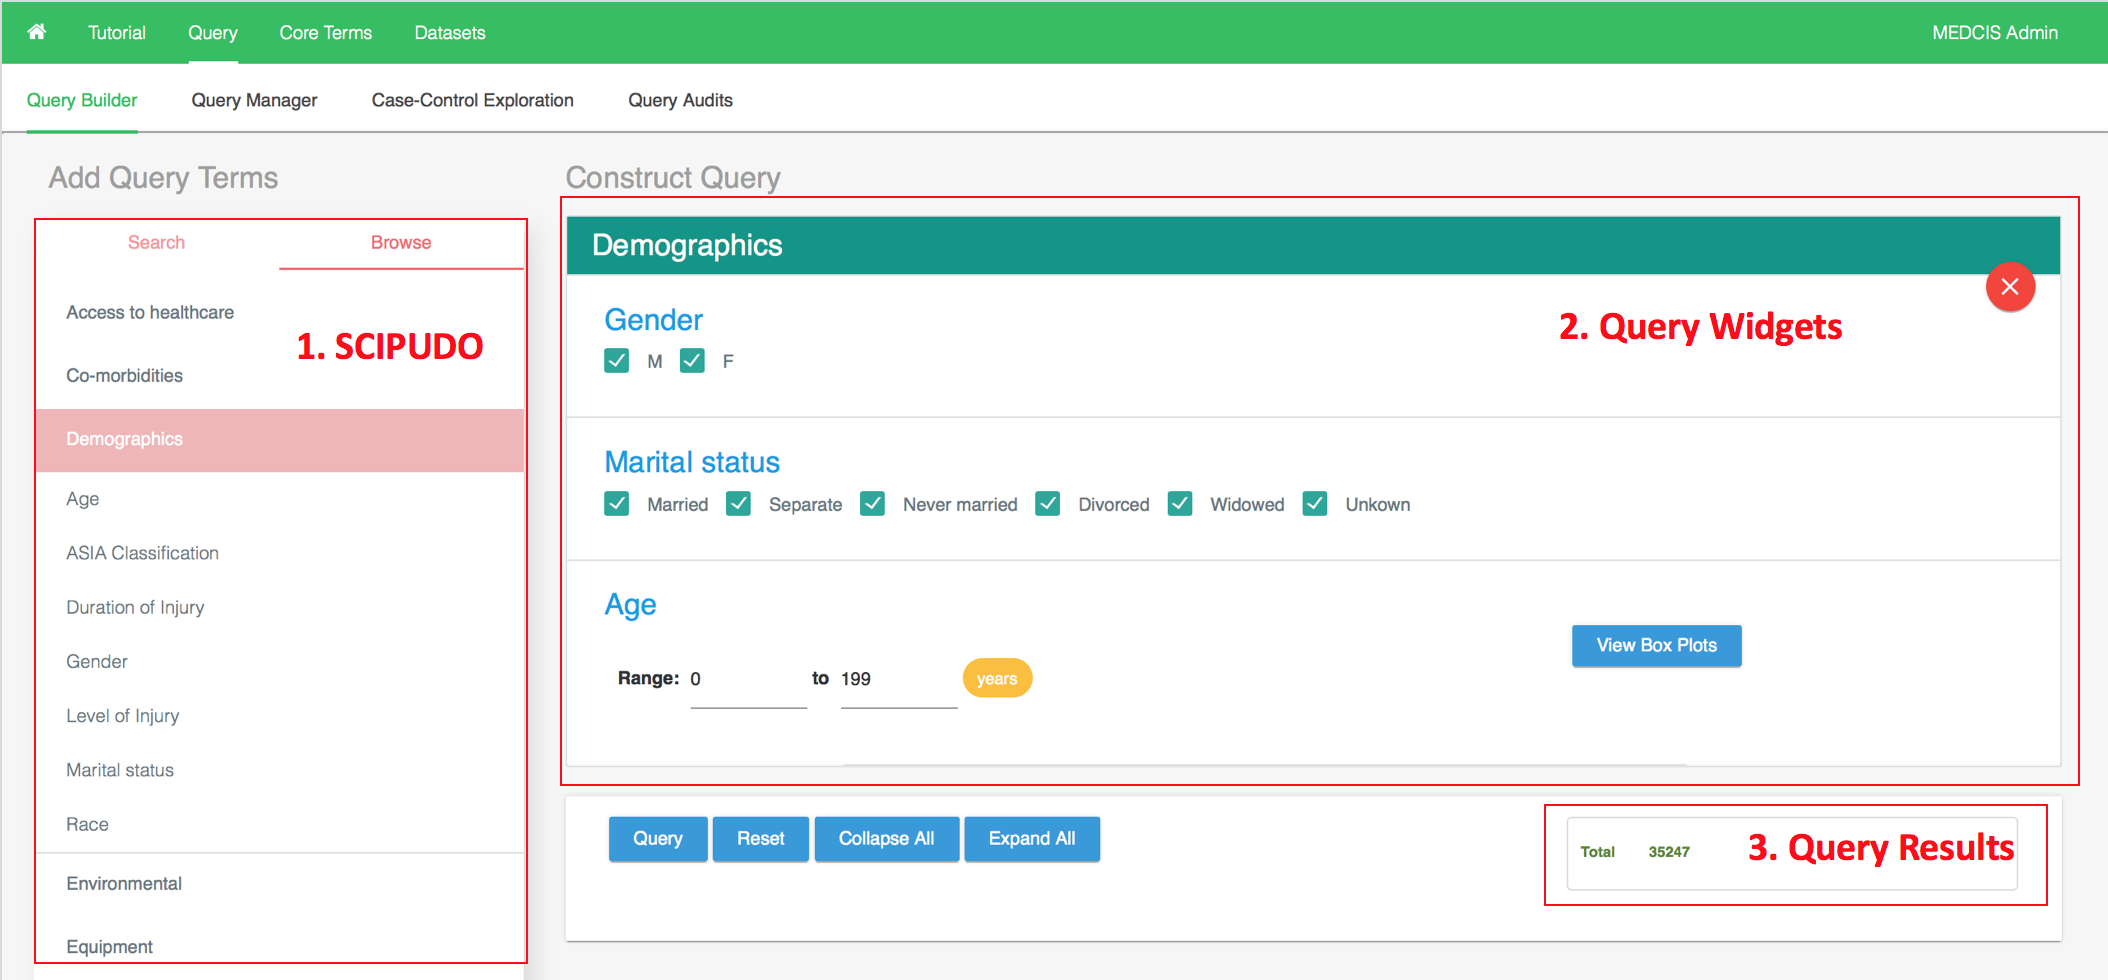
\includegraphics[scale=0.4]{pics/interface.png}
  \caption{SCIPUDSphere User Interface - Query Builder}
  \label{interface}
\end{figure}

\subsubsection{Query Builder}
Shown as below (Figure \ref{interface}), the query builder interface consists of a set of drop-down menus that are directly populated with the SCIPUDO classes. This allows users to flexibly construct queries. The query interface has been implemented using Rails 5.0, an agile web development framework and is integrated with SCIPUDSphere system, which provides an integrated environment for investigators for risk factors identification. The Query Manager saves queries for future reuse, which can be searched by keywords in title, description, or the query itself. We omit the description of Query Manager since the functionalities of this component is similar to that of an email management application.

\vspace{-3mm}
\begin{itemize}
\setlength\itemsep{0em}
  \item SCIPUDO is displayed in the form of a set of drop-down menus. There are two modes for user to build queris. One is browse mode, and the other is search mode. In the search mode, users can search specific risk factors by typing their names, while in the browser mode users can expand the drop-down menus to select risk factors.
  \item Query Widget is a set of criteria which will be translated into local database query langauge dynamically. User can interactively select domains they are interested in and determine numberic range by specify the bottom and top range. For example, the query in Figure \ref{interface} will be translated into: select patients whose age are between 0 to 199, who are male or female, and all marital status like married, separate and so. 
  \item Query Result will show the distince number of patients who statisfy the criteria built in the query widget. In this example, the query result is 35,247.
\end{itemize}
\vspace{-3mm}

\subsubsection{Graphical exploration}
The graphical exploration interface has been designed and implemented to support visual exploration of two risk factors (suppose x and y corresponding to x-axis and y-axis). There are bar plots and box plots in the graphical views. Bar plots are shown when the y-axis is a categorical type of data, and box plots are displayed when the y-axis is a numeric type of data. Such plots power users to have a better understanding of the data distribution of y against x.

\subsubsection{Case-control exploration}
The case-control exploration interface allows users to perform cross-cohort case-
control analyses. It provides a general template for users to build a case-control
exploration step by step. Step 1 is to set base query terms, where users can specify the criteria for base population (e.g., age between 45 and 85 years, race is American Indian or Alaska Native, and no history of AIDS). Step 2 is to set the condition for cases (e.g., bed type is standard). Step 3 is to set the condition for controls (e.g. bed type is hospital). Step 4 is to set the match terms (e.g., gender and marital status). Step 5 is to set outcome terms (e.g., level of injury). The result of the case-control exploration is displayed as a table with case and control counts for the match and outcome terms.


\section{Evaluation}
In this section, we evaluated SCIPUDSphere from data import, query performance. For data import, we recorded the time spent in importing data into MySQL. For query performance, we set up several sets of risk factors that are composed of single concepts as well as combined concepts to evaluate our query performance based on the query time.

All these evaluations are conducted on a computer consisted of Intel Core i5 processor and 8 GB RAM.
\subsection{Data Import Time}

Table 2 shows the import time for different datasets respectively. We only measured the actual import time necessary for performing the data import without considering the data preprocessing part. It is shown that importing risk data into our domain database took about several minutes which depend on the size of risk data to import.

\begin{table}[!ht]
\centering
\caption{Import Time}
  \begin{tabular}{|l|l|l|l|l|}
  \hline
    \textbf{Dataset}  & \textbf{Import time 1} & \textbf{Import time 2} & \textbf{Import time 3} & \textbf{Average} \\ \hline
    Demographic & 240.7s & 232.7s & 231.1s & 234.8s  \\ \hline
    Co-morbidities  & 930.3s & 934.7s & 928.7s & 913.2s  \\ \hline
    Patient SCI diagnosis  & 440.6s & 466.1s & 467.9s & 458.2s \\ \hline
  \end{tabular}
\end{table}

\subsection{Query Performance}
To evaluate our query performance using Mysql as the backend database, we conduct two sets of queries experiments on all the three datasets. The first set of queries consists of single risk factor while the concepts in the second set of queries are combined risk factors. As shown in Table 3, The query time for different set of risk factors remain relative fast even with more than 30,000 data records.

\begin{table}[!ht]
\centering
\caption{Query Performance of SCIPUDSphere User Interface}
  \begin{tabular}{|l|l|l|l|l|}
  \hline
    \textbf{Query Concepts}  & \textbf{Query Time 1} & \textbf{Query Time 2} & \textbf{Query Time 3} & \textbf{Average} \\ \hline
    Age & 0.349s & 0.412s & 0.356s & 0.372s \\ \hline
    Race & 0.449s & 0.415s & 0.451s & 0.438s \\ \hline
    Gender   & 0.411s & 0.412s & 0.432s & 0.418s \\ \hline
    Marital Status   & 0.269s & 0.249s & 0.276s & 0.264s \\ \hline
    Race, Gender, Age & 0.657s & 0.684s & 0.613s & 0.651s \\ \hline
  \end{tabular}
\end{table}

\section{Discussion}
SCIPUDSphere demonstrates the capability of extracting and integrating large scale of risk data. Besides, SCIPUDSphere user interface is a powerful, comprehensive risk factor data query interface. Utilizing MySQL as the domain database, our query interface can achieve fast query performance along with rich useful functions like graphical exploration, case-control exploration. Users can sign up in our interface, save their queries, retrieve and redo these queries afterward. 

One limitation in the SCIPUDSphere system is that we use traditional relational database as our domain database, which could potentially be improved by using NoSQL databases. Besides, in current stage, we only extracted three main categories data, which are demographics, co-morbidities, and patient SCI diagnosis data respectively. Our ultimate goal is to extract, integrate all the targeted data from VINCI to our SCIPUDSphere system, and to creat the environmental, social and clinical domain database. Then we can perform a more comprehensive and systematic evaluations, including usability evaluation. 

\section{Conclusion}
In this paper, we introduce a bioinformatics platform, called SCIPUDSphere, to enable data extraction, storage, and analysis to provide clinical decision support and user interface providing access to well-annotated and de-identified data generated from multiple domains. We created a dedicated Spinal Cord Injury Pressure Ulcer and Deep tissue injury ontology (SCIPUDO) as the knowledge resource for processing specialized terms related to SCI, PU and DTI. We extracted the demographics, co-morbidities, and patient SCI diagnosis data from VINCI. Besides, through adapting existing tools: Physio-MIMI and OnWARD, we successfully implemented a powerful and intuitive user interface that empowers researchers to quickly pinpoint the desired risk factor and perform exploratory query.

SCIPUDSphere is rather promising, given its ability in scaling well with the data volume and efficiently querying risk factor data. We notice that choosing MySQL as our backend database do guarantee fast and reliable query performance.

% For future development, we will explore more NoSQL databases like Hadoop Hbase and compare their performance with MongoDB. Doing so, we hope to add more options to grappling with large-scale sleep data and explore more Big Data solutions to help sleep research community to advance with the rapidly increasing sleep data and provide enough computational power.

\textbf{ACKNOWLEDGMENTS}\\
The authors thank the University of Kentucky Center for Clinical and Translational Science (Clinical and Translational Science Award UL1TR001998), as well as........

\makeatletter
\renewcommand{\@biblabel}[1]{\hfill #1.}
\makeatother



{\footnotesize
\bibliographystyle{unsrt}
\begin{thebibliography}{1}
\setlength\itemsep{-0.1em}

\bibitem{ref1}
Langemo DK, Melland H, Hanson D, Olson B, Hunter S. The lived experience of having a pressure ulcer: A qualitative analysis. Adv Skin Wound Care. 2000;13(5):225-35.
\bibitem{ref2}
Clark FA, Jackson JM, Scott MD, Carlson ME, Atkins MS, Uhles-Tanaka D, Rubayi S. Data-based models of how pressure ulcers develop in daily-living contexts of adults with spinal cord injury. Arch Phys Med Rehabil. 2006;87(11):1516-25.
\bibitem{ref3}
Henzel MK, Bogie KM, Guihan M, Ho CH. Pressure ulcer management and research priorities for patients with spinal cord injury: Consensus opinion from SCI QUERI Expert Panel on Pressure Ulcer Research Implementation. J Rehabil Res Dev. 2011;48(3):xi–xxxii.
\bibitem{ref4}
Lyder CH, Ayello EA. Pressure ulcers: a patient safety issue. In: Hughes RG, ed. Patient Safety and Quality: An Evidence-Based Handbook for Nurses. AHRQ Publication No. 08-0043. Rockville, MD: Agency for Healthcare Research and Quality 2008:1–33.
\bibitem{ref5}
Reddy M, Gill S, Rochon P. Preventing pressure ulcers: a systematic review. JAMA 2006;296(8):974–84.
\bibitem{ref6}
National Pressure Ulcer Advisory Panel, European Pressure Ulcer Advisory Panel and Pan Pacific Pressure Injury Alliance. Prevention and Treatment of Pressure Ulcers: Clinical Practice Guideline, 2014.
\bibitem{ref7}
Oomens CW, Loerakker S, Bader DL. The importance of internal strain as opposed to interface pressure in the prevention of pressure related deep tissue injury. J Tissue Viability. 2010;19(2):35-42.
\bibitem{ref8}
Oot-Giromini B, Bidwell FC, Heller NB, et al. Pressure ulcer prevention versus treatment, comparative product cost study. Decubitus. 1989;2(3):52–4.
\bibitem{ref9}
Panel on the Prediction and Prevention of Pressure Ulcers in Adults. Pressure ulcers in adults: prediction and prevention Clinical Practice Guideline No 3 . Rockville, MD: Agency for Health Care Policy and Research; 1992. AHCPR Publication No 92-0047.
\bibitem{ref10}
Kosiak M. Prevention and rehabilitation of pressure ulcers. Decubitus 1991;4(2):60–2 4, 6 passim
\bibitem{VINCI}
https://www.hsrd.research.va.gov/for\_researchers/vinci/

\bibitem{physiomimi}
Zhang G-Q, Siegler T, Saxman P, et al. VISAGE: A Query Interface for Clinical Research. Summit on Translational Bioinformatics. 2010;2010:76-80.
\bibitem{onward}
Tran V-A, Johnson N, Redline S, Zhang G-Q. OnWARD: Ontology-driven Web-based Framework for Multi-center Clinical Studies. Journal of biomedical informatics. 2011;44(Suppl 1):S48-S53. doi:10.1016/j.jbi.2011.08.019.
\bibitem{ref11}
Liu, Y.;Wang, Y.; Jin, Y. Research on the improvement of MongoDB Auto-Sharding in cloud environment. In Proceedings of 7th International Conference on Computer Science \& Education (ICCSE), Melbourne, Australia, 14–17 July 2012; pp. 851–854.
\bibitem{ref12}
Kanade, A.; Gopal, A.; Kanade, S. A study of normalization and embedding in MongoDB. In Proceedings of the 2014 IEEE International Conference on Advance Computing Conference (IACC), Gurgaon, India, 21–22 February 2014; pp. 416–421.
\bibitem{ref13}
Cui L, Huang Y, Tao S, Lhatoo SD, Zhang GQ. ODaCCI: Ontology-guided Data Curation for Multisite Clinical Research Data Integration in the NINDS Center for SUDEP Research. AMIA Annual Symp Proc 2016, pp. 441-450.
\bibitem{ref14}
National Sleep Research Resource. https://sleepdata.org/datasets.
\bibitem{ref15}
Aniceto R, Xavier R, Guimarães V, et al. Evaluating the Cassandra NoSQL Database Approach for Genomic Data Persistency. International Journal of Genomics. 2015;2015:502795. doi:10.1155/2015/502795.
\bibitem{ref16}
Dinov ID, Heavner B, Tang M, et al. Predictive Big Data Analytics: A Study of Parkinson’s Disease Using Large, Complex, Heterogeneous, Incongruent, Multi-Source and Incomplete Observations. Draganski B, ed. PLoS ONE. 2016;11(8):e0157077. doi:10.1371/journal.pone.0157077.

\end{thebibliography}
}
\end{document}
